\documentclass[11pt]{article}

\usepackage[top=1in, bottom=1in, includefoot]{geometry} %use to adjust margins
\usepackage{fancyhdr} %use to create custom header and footer
\usepackage{graphicx} %use to import graphics
\usepackage{float} %use to align graphics
\usepackage[none]{hyphenat} %prevents hypenation
\usepackage{amsfonts, amsmath, amssymb} %for typesetting math
\usepackage[nottoc,notlot,notlof]{tocbibind} %table of contents

\pagestyle{fancy}
\fancyhead{} %clear default header
\fancyfoot{} %clear default footer
\fancyhead[L]{\slshape \MakeUppercase{Place Title Here}}
\fancyfoot[C]{\thepage}  %place page number in center
%\renewcommand{\headrulewidth}{0pt} %remove line in header
\renewcommand{\footrulewidth}{0pt} %remove line in footer

\setlength{\parindent}{4em}
%\setlength{\parskip}{1em}
\renewcommand{\baselinestretch}{1.25} %line spacing

\parindent 0ex %remove paragraph indent

\begin{document}

\begin{titlepage} %custom title page
	\begin{center}
	\vspace*{1cm}
	\Large{\textbf{IB Mathematics SL}}\\
	\Large{\textbf{Internal Assessment}}\\
	\vfill
	\line(1,0){400}\\
	[1mm]
	\huge{\textbf{This is a Sample Title}}\\
	[3mm]
	\Large{- This is a Sample Subtitle -}\\
	[1mm]
	\line(1,0){400}\\
	\vfill
%	By Student Name\\ %	DO NOT INCLUDE YOUR NAME
%	Candidate \# \\ %DO NOT INCLUDE YOUR CANDIDATE NUMBER
	\today \\
	\end{center}
\end{titlepage}

\tableofcontents
\thispagestyle{empty} %remove header and footer from this page
\clearpage

\setcounter{page}{1}

\section{Introduction}

Your aim and rationale must be clearly defined in your introduction \cite{DBHS1}. Your aim tells the reader what you are hoping to accomplish (you may find it helpful to phrase this in the form of a question) in this exploration, and the rationale tells the reader why this is important. You could consolodate the aim and rationale into a single sentence: ``In this exploration, I aim to \line(1,0){50}\, in order to \line(1,0){50}.'' Or, you can desribe them separately, like so: ``The aim of this investigation is to \line(1,0){50}. This is an important topic because \line(1,0){50}.'' \\

The introduction is a good place to let the reader know why your topic is personally relevant to YOU. This will help to establish some personal engagement\footnote{An example footnote}, which you will develop further throughout the work. You may write in first person, which will also help convey your original ideas. Remember, this is not a formal research paper. This is an informal personal exploration.\\

\section{Scoring Criterion} 
\subsection{Communication}
This criterion assesses the organization and coherence of the exploration. A well-organized exploration includes an introduction, has a rationale (which includes explaining why this topic was chosen), describes the aim of the exploration and has a conclusion. A coherent exploration is logically developed and easy to follow. Graphs, tables and diagrams should accompany the work in the appropriate place and not be attached as appendices to the document.\cite{DBHS2}\\

To score highly, you must clearly explain all steps, ideas, and concepts. Focus on your aim and avoid irrelevant discussion. Avoid repetitive calculations. Discuss all pictures, graphs, tables, and equations at the point where they occur in the work.

\subsection{Mathematical Presentation}
This criterion assesses to what extent the student is able to use appropriate mathematical language (notation, symbols, terminology), define key terms where required, and use multiple forms of mathematical representation such as formulas, diagrams, tables (see table \ref{tab:data1}), charts, graphs and models, where appropriate.\\ 

\begin{table}[H]
	\centering
		\begin{tabular}{|c | c | c | c |} \hline
			$x$ & 0 & 1 & 2\\ \hline
			$f(x)$ & 3 & 6 & 9\\ \hline
		\end{tabular}
	\caption{Caption goes here \protect\footnotemark}
	\label{tab:data1}
\end{table}
\footnotetext{This example shows how to include a footnote in a caption.}

Students are encouraged to use appropriate technology such as graphing calculators, screenshots, graphing apps (see figure \ref{fig:squeeze}), spreadsheets, databases, drawing and word-processing software, as appropriate, to
enhance mathematical communication. \\

To score highly, you must use appropriate mathematical language (i.e., use ``substitute'' instead of ``plug in''), define key terms, and express your results to an appropriate degree of accuracy (be sure to discuss your choice of accuracy).

\begin{figure}[H]
	\centering
	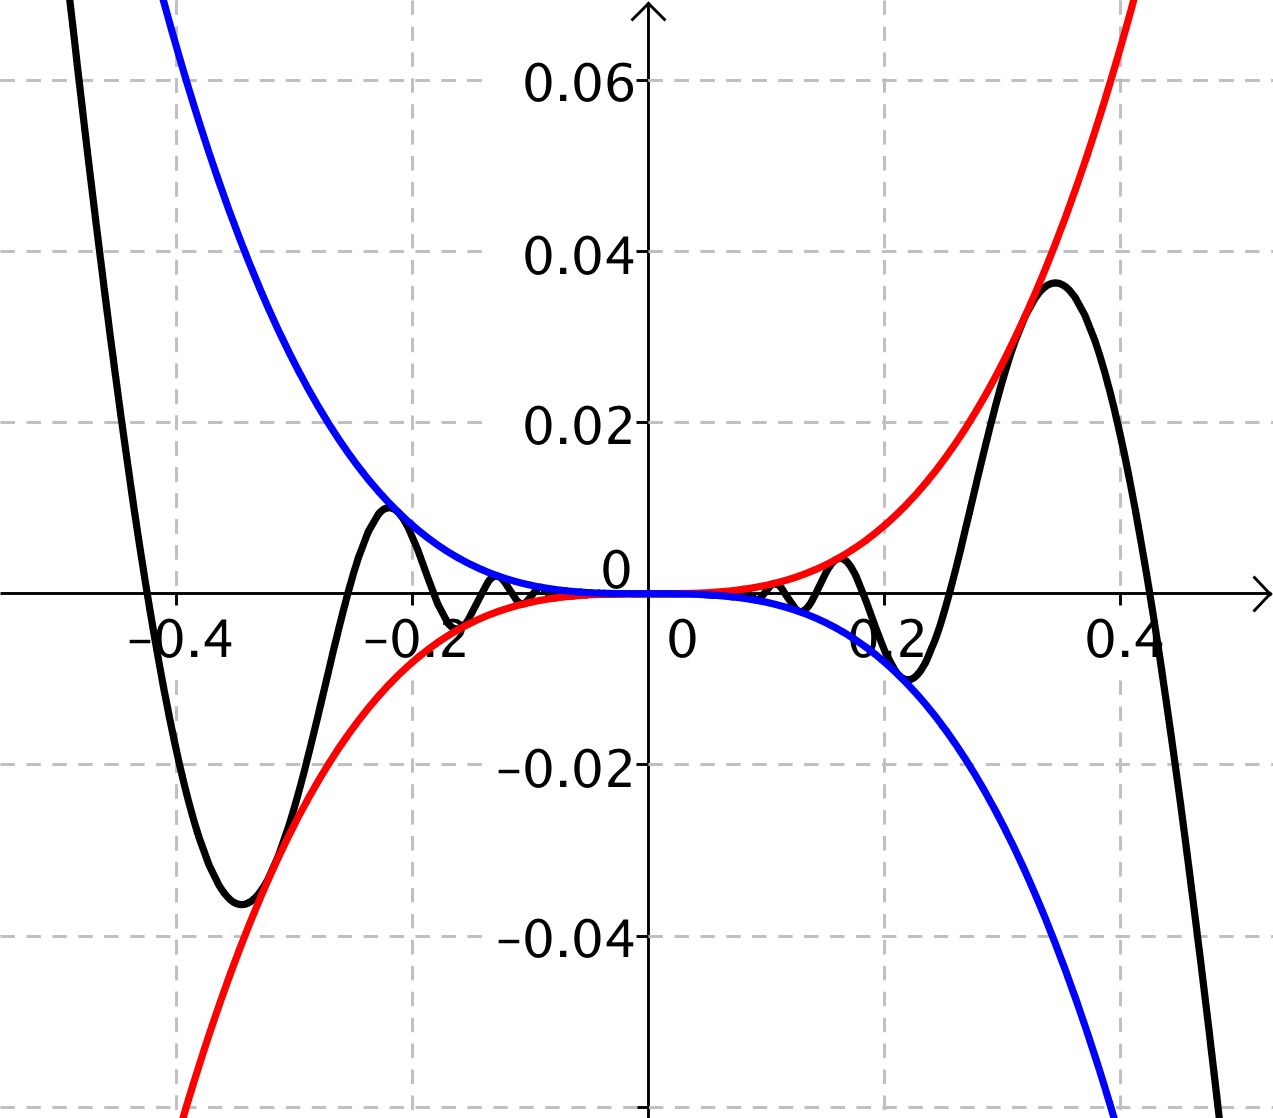
\includegraphics[scale=0.5]{limit}
	\caption{The Squeeze Theorem \cite{DBHS2}}
	\label{fig:squeeze}
\end{figure}

\subsection{Personal Engagement}
This criterion assesses the extent to which the student engages with the exploration and makes it their own. Personal engagement may be recognized in different attributes and skills. These include thinking independently and/or creatively, addressing personal interest and presenting mathematical ideas in their own way.\\

To receive full marks, students must show evidence of outstanding personal engagement. This includes making and testing conjectures. The work should be original. It may be from historical ideas and real world situations (for example, socio-economic, political awareness). Students should create some examples or present some ideas explained in depth.

\subsection{Reflection}
This criterion assesses how the student reviews, analyses and evaluates the exploration. Although reflection may be seen in the conclusion, it should also be found throughout the work. Identify and address issues as the piece develops, discuss limitations of the work where applicable, provide ideas for extensions, and reflect on the significance of the findings.

\subsection{Use of Mathematics}
This criterion assesses to what extent and how well students use mathematics in the exploration. Students are expected to produce work that is commensurate with the level of the course. The mathematics explored should either be part of the syllabus, or at a similar level or beyond. If the level of mathematics is not commensurate with the level of the course, a maximum of two marks can be awarded for this criterion.\\

The mathematics can be regarded as correct even if there are occasional minor errors as long as they do not detract from the flow of the mathematics or lead to an unreasonable outcome. Sophistication in mathematics may include understanding and use of challenging mathematical concepts, looking at a problem from different perspectives and seeing underlying structures to link different areas of mathematics. Rigour involves clarity of logic and language when making mathematical arguments and calculations. Precise mathematics is error-free and uses an appropriate level of accuracy at all times.

\section{Conclusion}
The exploration is intended to be an opportunity for students to use mathematics to develop an area of interest to them rather than merely to solve a problem set by someone else. Criterion C (personal engagement) will be looking at how well the student is able to demonstrate that he or she has “made the exploration their own” and expressed ideas in an individual way. \\

A total length of 6 - 12 pages should be appropriate. A common failing of mathematical writing is excessive repetition, and this should be avoided, as such explorations will be penalized for lack of conciseness. However, it is recognized that some explorations will require the use of several diagrams, which may extend them beyond the page limit.\\

\section{Using \LaTeX}
Be sure to cite any sources you use throughout the text. See the references section in the \TeX\, file for samples of MLA citations for books\cite{name1}, articles\cite{name2}, journals\cite{name3}, websites\cite{name4}, and images\cite{name5}. Replace ``name1'', ``name2'', etc. with appropriate keywords. There are more advanced methods of creating bibliographies, but the method used here is simplest for a short list of references.\\

Also note that you may have to compile the document twice before you see updated citations and the updated table of contents. 

\pagebreak[4]
\begin{flushleft}
\begin{thebibliography}{}

\bibitem{DBHS1} 
Alcosser, Howard. 
``Diamond Bar High School.''
\textit{Internal Assessment : Mathematical Exploration}. 
Web. 27 May 2015.
\texttt{<http://dbhs.wvusd.k12.ca.us/ourpages/auto/\\2010/10/1/38060822/INTERNAL\%20ASSESSMENT\_handout.pdf>.}

\bibitem{DBHS2} 
Alcosser, Howard. 
``Diamond Bar High School.'' 
\textit{Mathematical Exploration Rubric}. 
Web. 27 May 2015.
\texttt{<http://dbhs.wvusd.k12.ca.us/ourpages/auto/2010/10/1/38060822/\\IA\_2014\_rubric.pdf>.}

\bibitem{name1} %book
Lastname, Firstname. 
\textit{Title of Book.} 
City of Publication: 
Publisher, 
Year of Publication. 
Medium of Publication. %ex: Print.

\bibitem{name2} %magazine article
Author(s). 
``Title of Article.'' 
Title of Periodical 
Day Month Year: 
pages. 
Medium of publication.

\bibitem{name3} %journal article
Author(s). 
``Title of Article.'' 
Title of Journal 
Volume.Issue (Year): 
pages. 
Medium of publication.

\bibitem{name4} %website
Editor, author, or compiler name (if available). 
\textit{Name of Site.} 
Name of institution or organization affiliated with the site (sponsor or publisher), 
date of resource creation (if available). 
Medium of publication. 
Date of access.
\texttt{<http://www.samplewebsite.com>.}

\bibitem{name5} %image
Artist's name, 
\textit{The Work of Art}, 
Date of creation, 
Institution and city where the work is housed. 
\textit{Name of  Website}, 
Medium of publication, 
Date of access.

\end{thebibliography}
\end{flushleft}

\end{document}